\documentclass{scrartcl}
\setcounter{tocdepth}{4}
\setcounter{secnumdepth}{4}
\usepackage[utf8]{inputenc}
\usepackage{graphicx} 
\usepackage{tabularx}
\usepackage{listings}
\usepackage{float}
\usepackage{pdfpages}
\usepackage{xcolor}
\usepackage{scrpage2}
\usepackage{tikz}
\usepackage[top=3.5cm, bottom=2.5cm, left=2.5cm, right=2.5cm,headheight=110pt]{geometry}

\title{Anperi}
\subtitle{Projektmanagement\\ Projektabschlussbericht \\  SS2018 - AI 6}
\author{Jannes Peters - 590252 \\ Adrian Kurth - 590289 \\ Jesse Nis Arff - 590245}
\date{22.06.2018}

\begin{document}

\maketitle
\newpage
\renewcommand\contentsname{Inhalt}
\tableofcontents{}
\newpage

\pagestyle{scrheadings}
\addtolength{\voffset}{-15pt}
\ihead{\textbf{Projektmanagement}}  
\chead{Projekt: Anperi \\ Dok.-Typ: Projektabschlussbericht}
\ohead{Datum: 22.06.2018}
\setheadsepline{0.4pt}

\section{Projektsteckbrief}
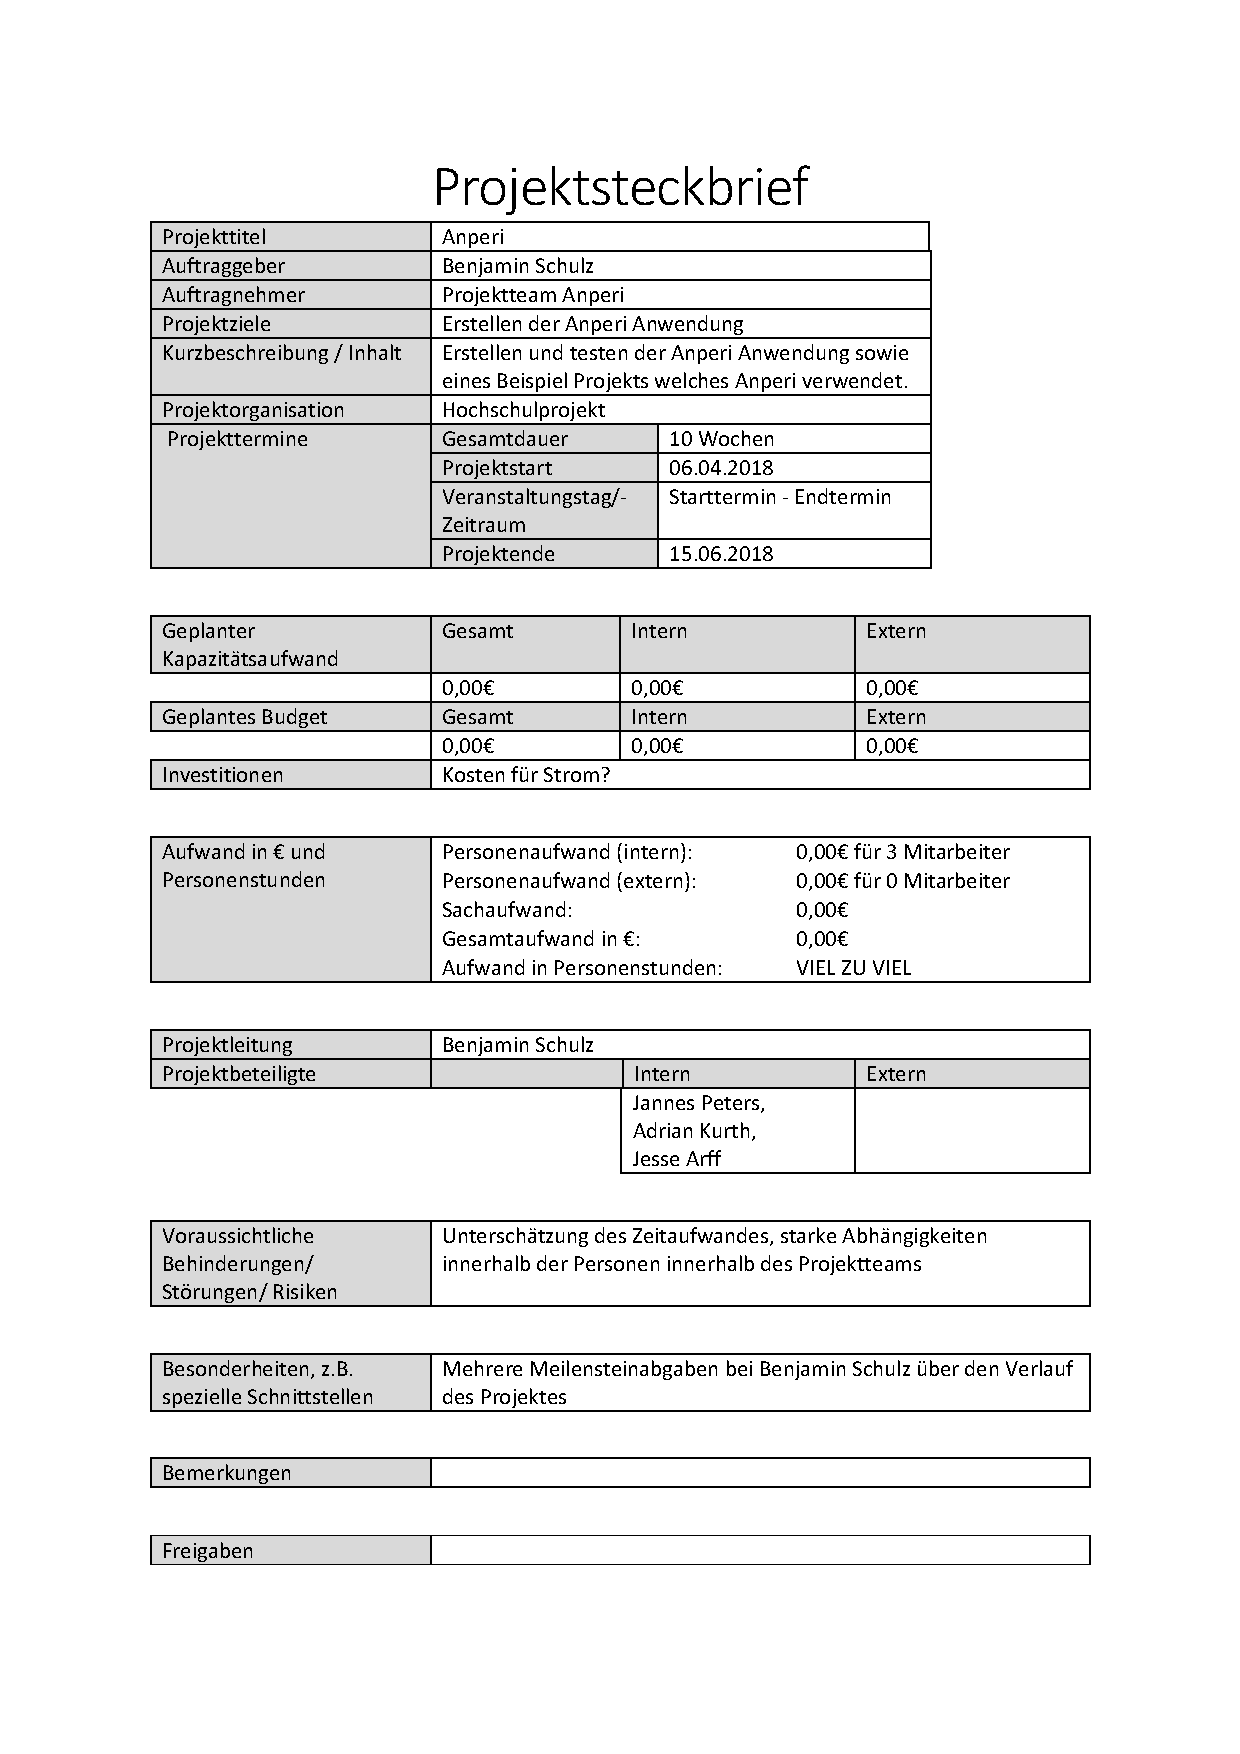
\includegraphics[scale=0.75]{Projektsteckbrief.pdf}
\includepdf[pages=2-, scale=0.75, pagecommand={\pagestyle{scrheadings}}]{Projektsteckbrief.pdf}

\section{Personenverteilung}
\subsection{Organigramm}
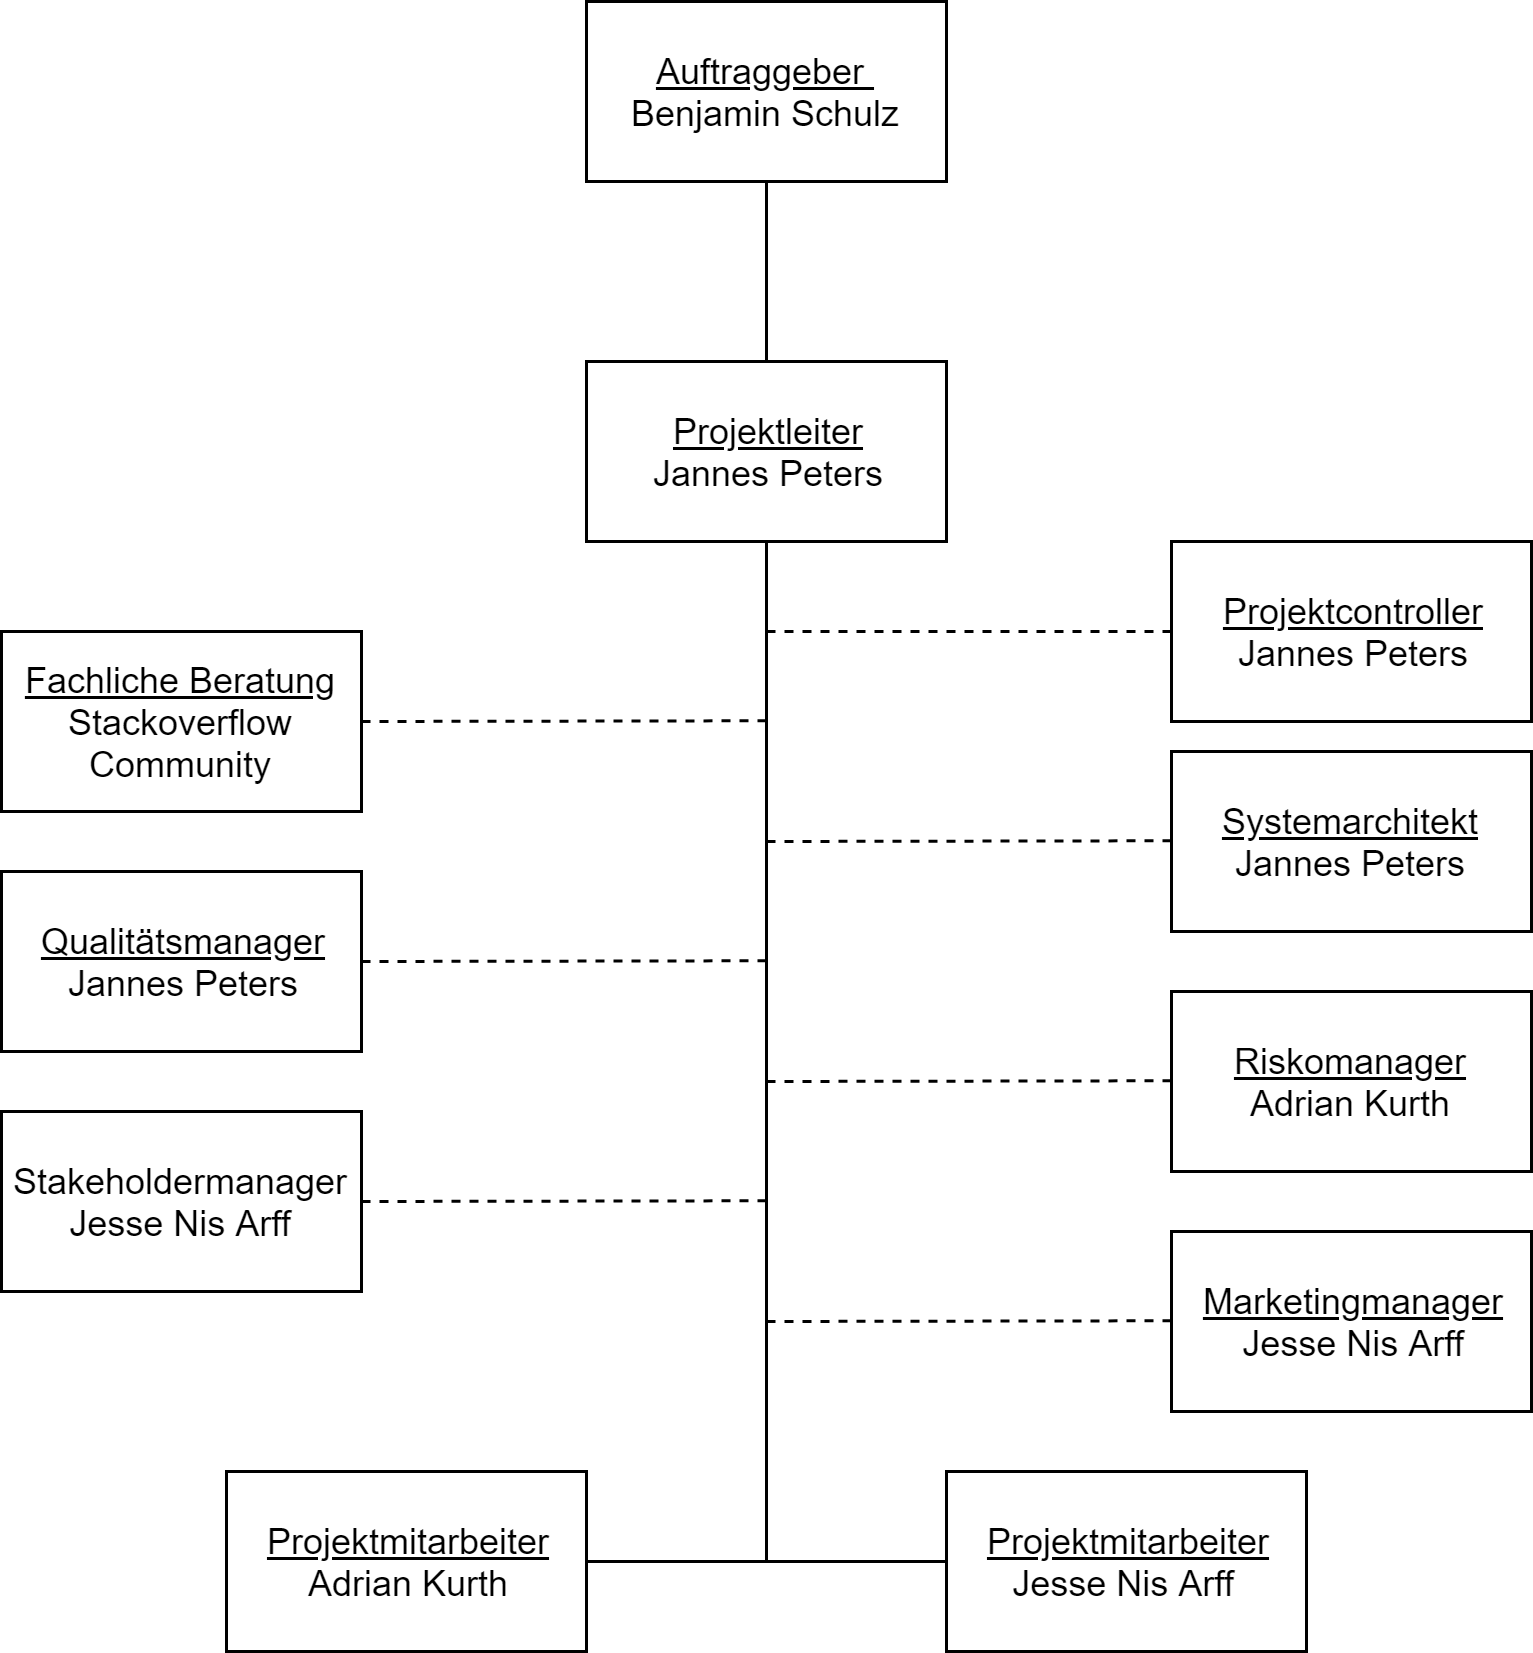
\includegraphics[scale=0.3]{Organigramm.png}
\subsection{Verantworlichtkeitsmatrix}
\begin{center}
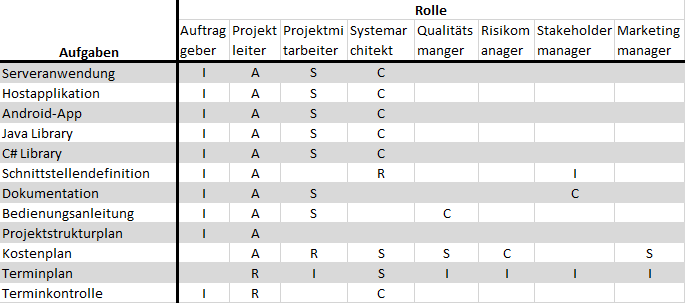
\includegraphics[scale=0.7]{RASCI.png}
\end{center}
\section{Phasenplan und Meilensteine}
\subsection{Phasenplan}
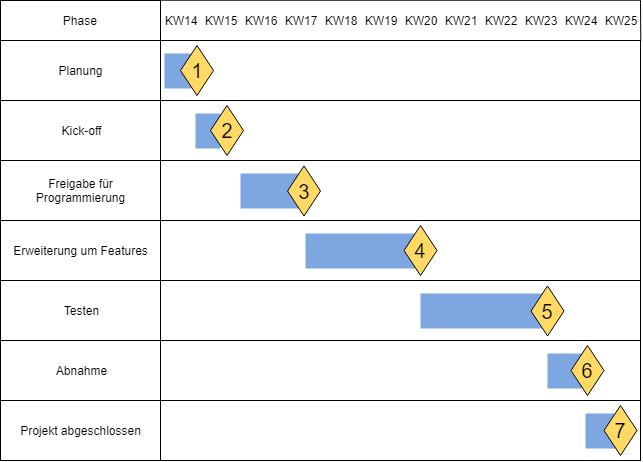
\includegraphics[scale=0.75]{Phasen.png}
\subsection{Meilensteine}
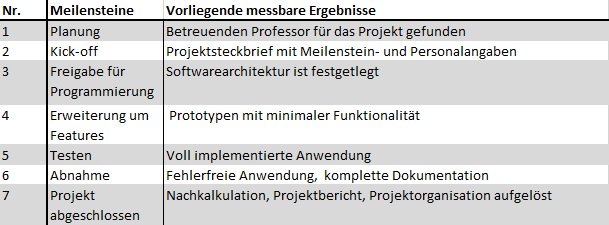
\includegraphics[scale=0.75]{Meilensteine.png}
\section{Projektstrukturplan}
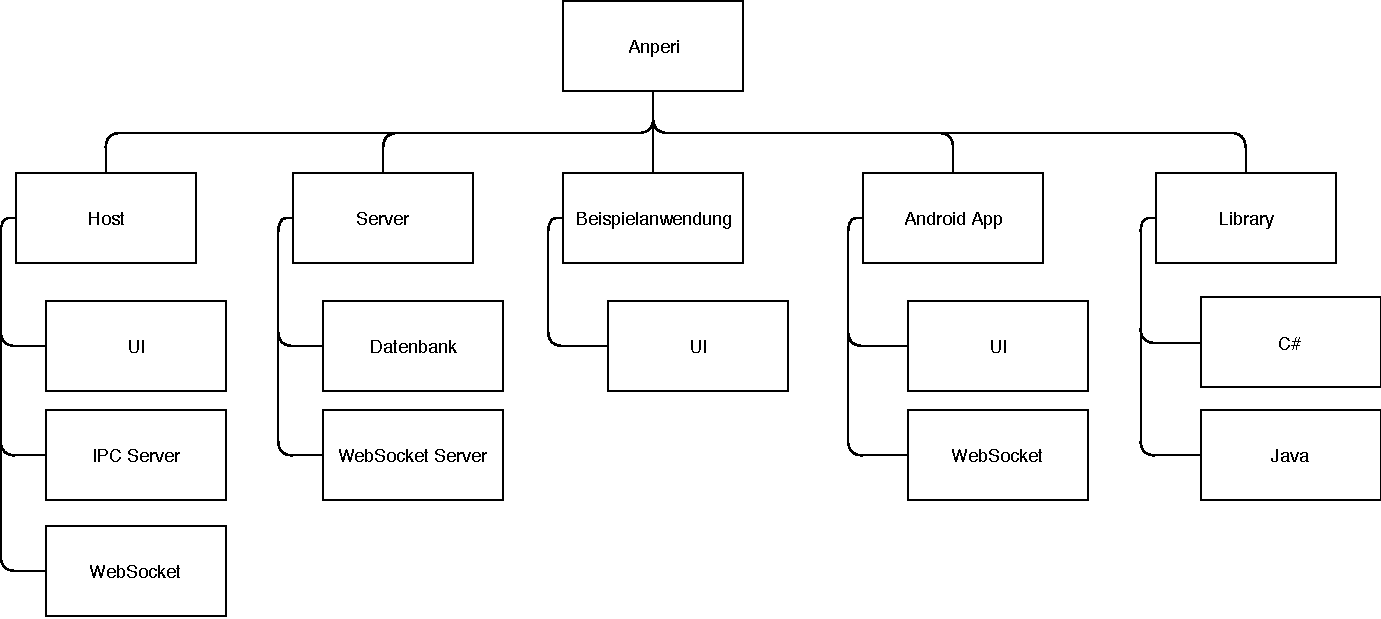
\includegraphics[scale=0.75]{PSP.pdf}
\section{Arbeitspaketbeschreibungen}
\subsection{Projekt suchen}
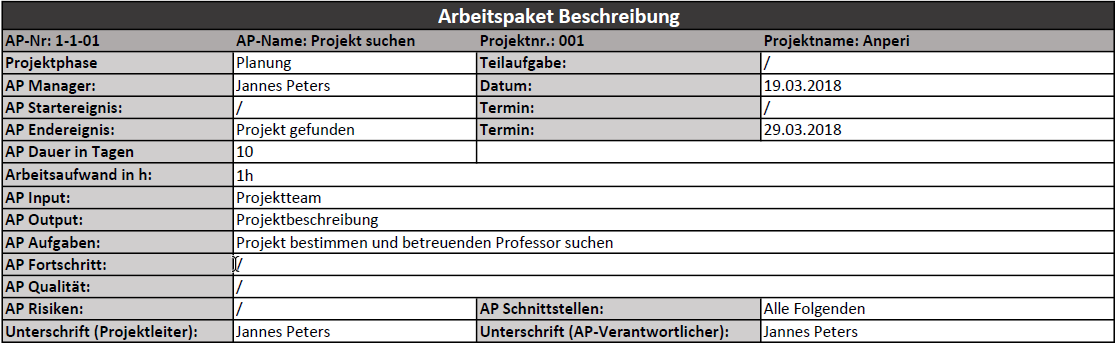
\includegraphics[scale=0.6]{ArbeitsPakete/AP1-1-01.png}
\subsection{Host}
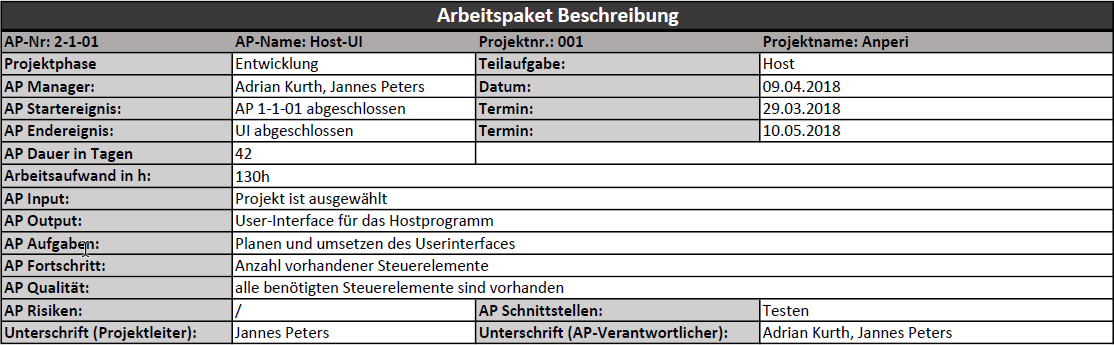
\includegraphics[scale=0.6]{ArbeitsPakete/AP2-1-01.png}
\\
\\
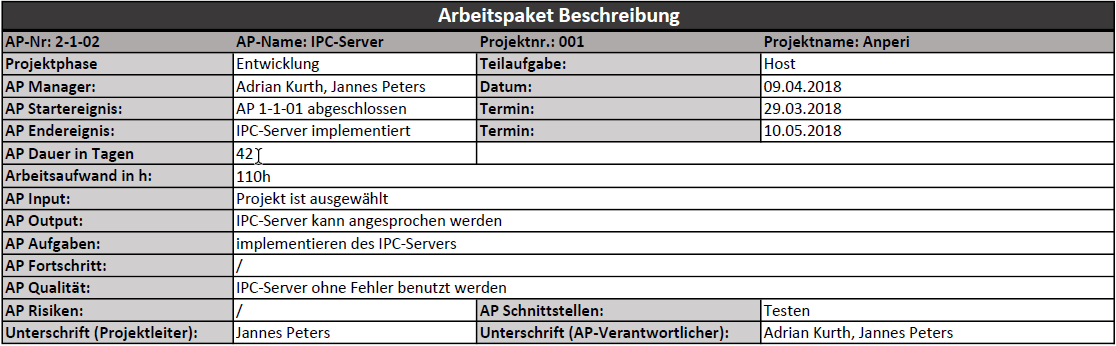
\includegraphics[scale=0.6]{ArbeitsPakete/AP2-1-02.png}
\\
\\
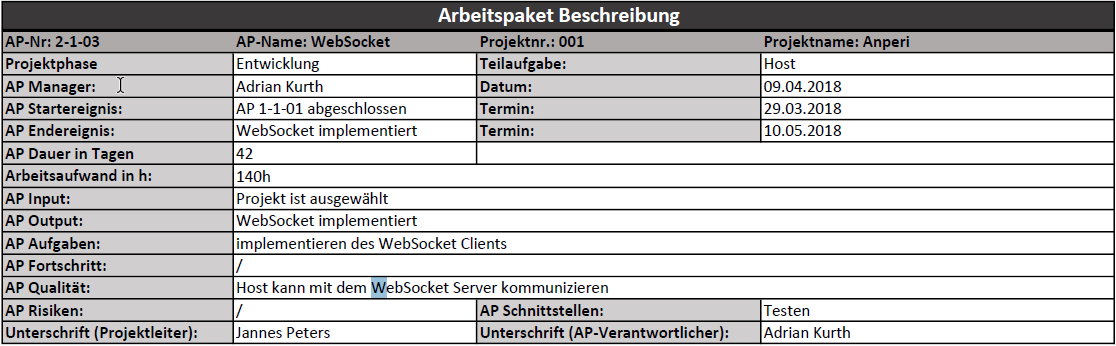
\includegraphics[scale=0.6]{ArbeitsPakete/AP2-1-03.png}
\subsection{Server}
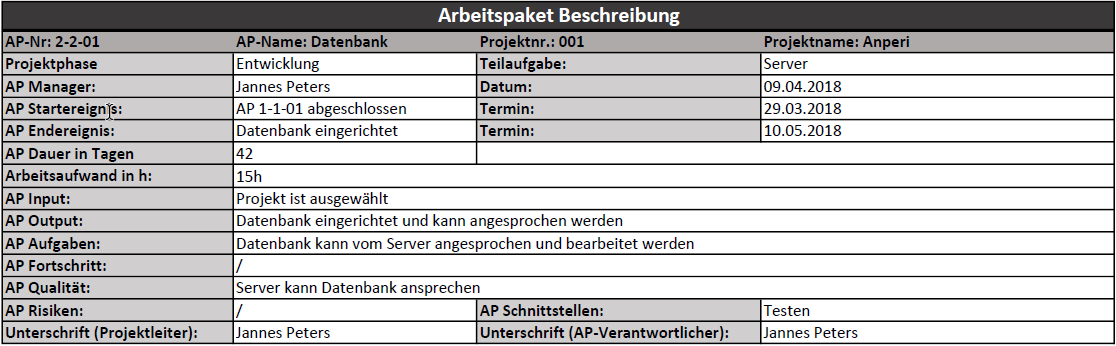
\includegraphics[scale=0.6]{ArbeitsPakete/AP2-2-01.png}
\\
\\
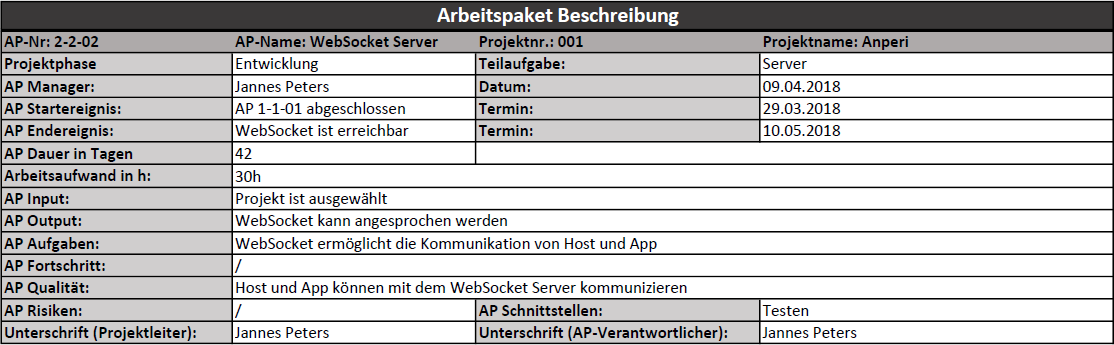
\includegraphics[scale=0.6]{ArbeitsPakete/AP2-2-02.png}
\subsection{Beispielprogramm}
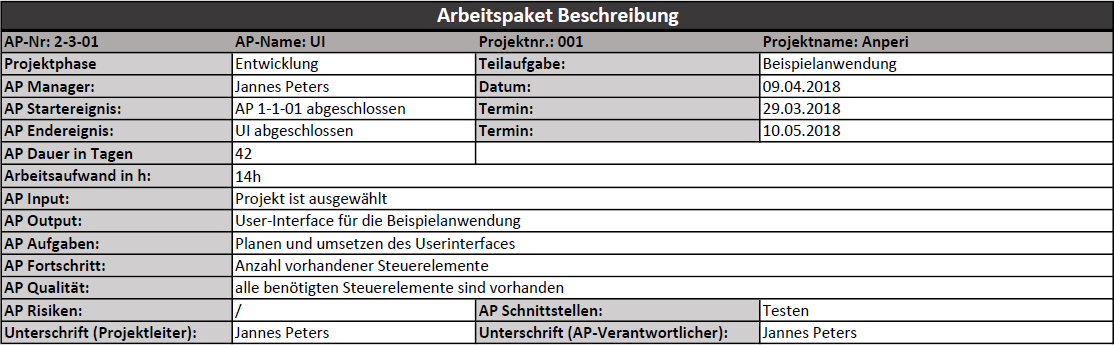
\includegraphics[scale=0.6]{ArbeitsPakete/AP2-3-01.png}
\subsection{Android-App}
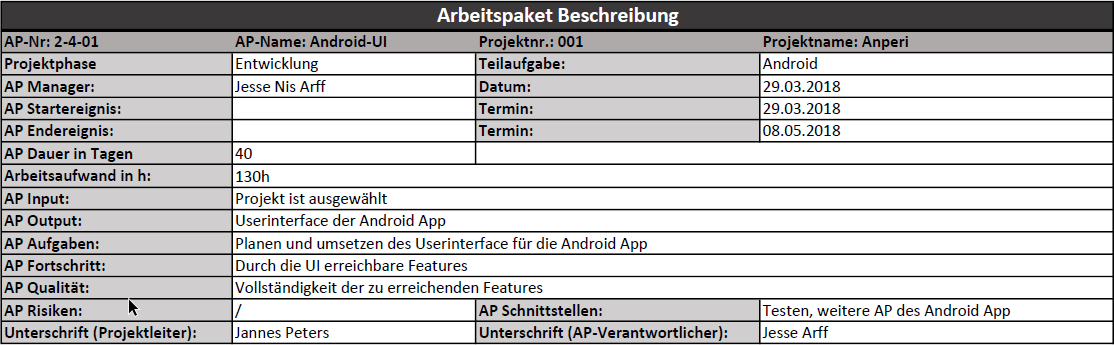
\includegraphics[scale=0.6]{ArbeitsPakete/AP2-4-01.png}
\\
\\
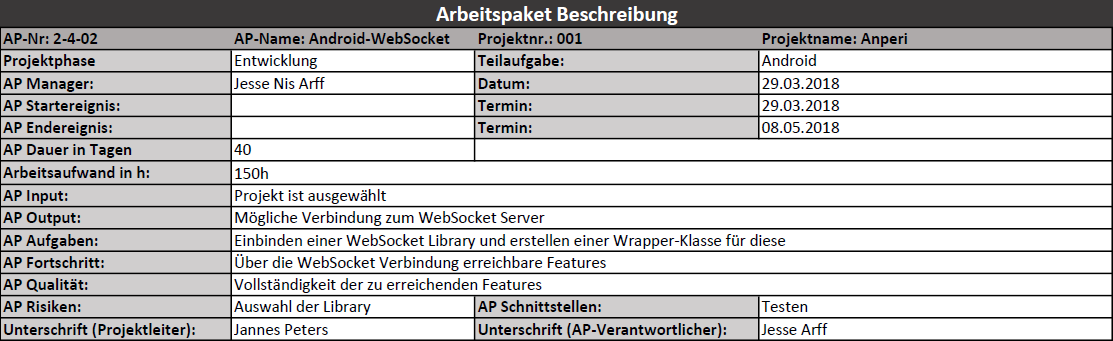
\includegraphics[scale=0.6]{ArbeitsPakete/AP2-4-02.png}
\\
\\
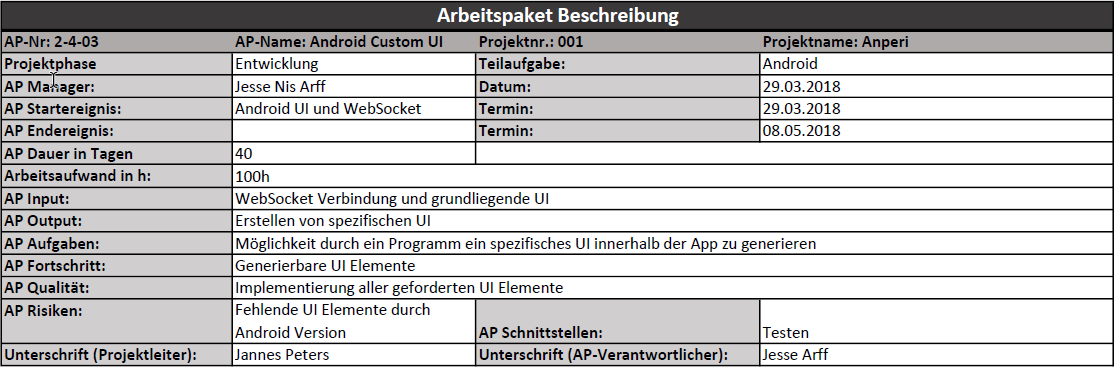
\includegraphics[scale=0.6]{ArbeitsPakete/AP2-4-03.png}
\subsection{Library}
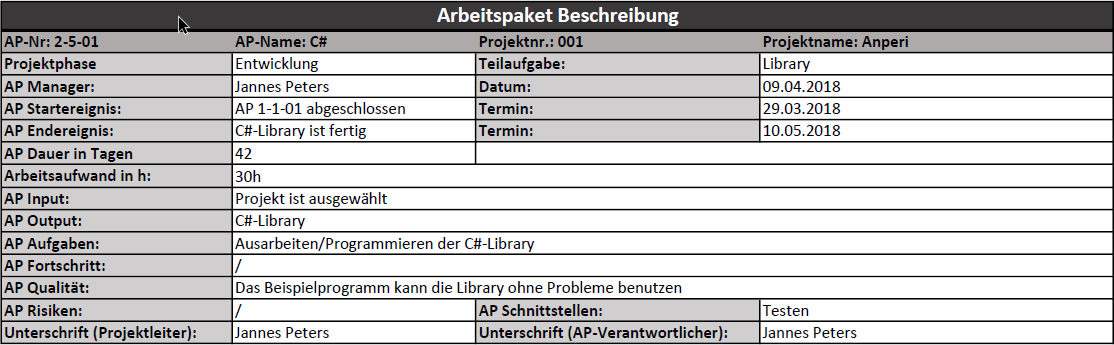
\includegraphics[scale=0.6]{ArbeitsPakete/AP2-5-01.png}
\\
\\
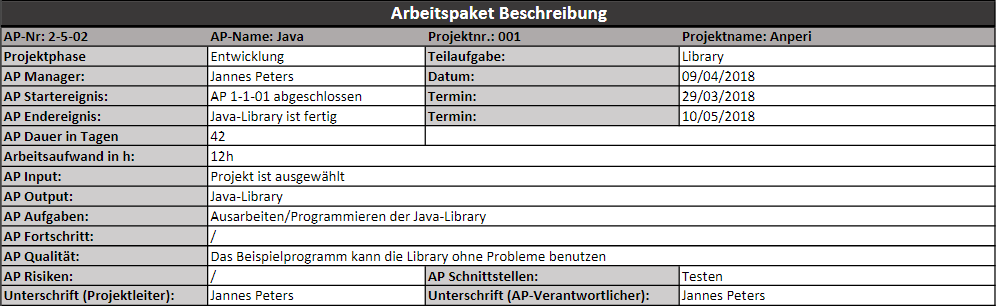
\includegraphics[scale=0.672]{ArbeitsPakete/AP2-5-02.png}
\\
\\
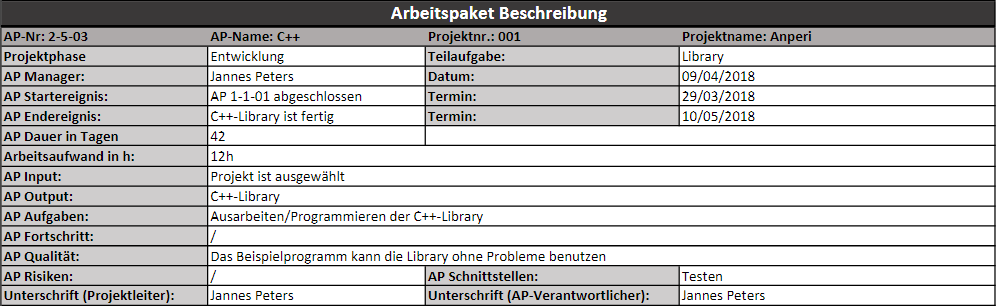
\includegraphics[scale=0.672]{ArbeitsPakete/AP2-5-03.png}
\subsection{Testen}
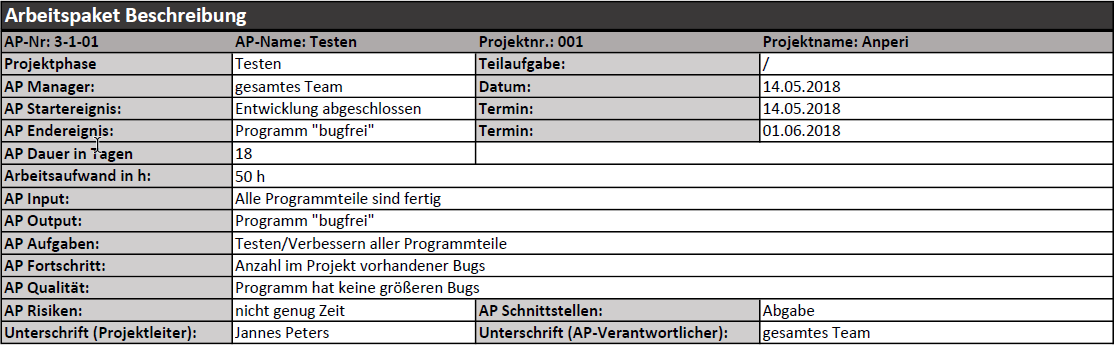
\includegraphics[scale=0.6]{ArbeitsPakete/AP3-1-01.png}
\subsection{Abgabe}
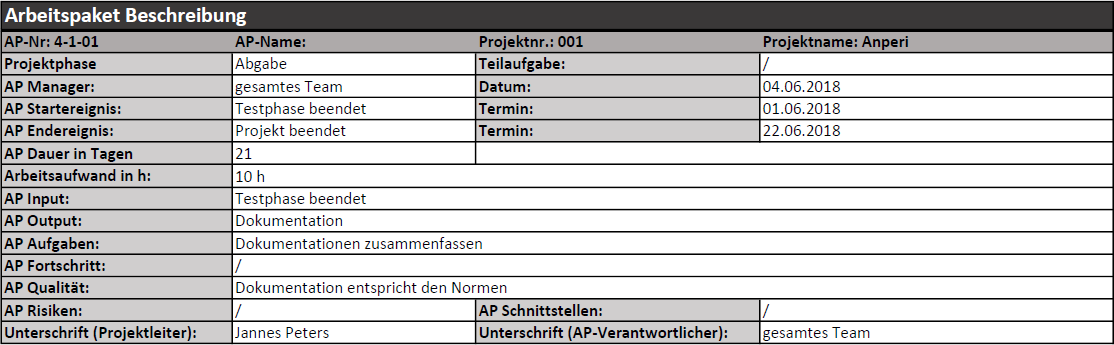
\includegraphics[scale=0.6]{ArbeitsPakete/AP4-1-01.png}
\subsection{Änderungsaufträge}
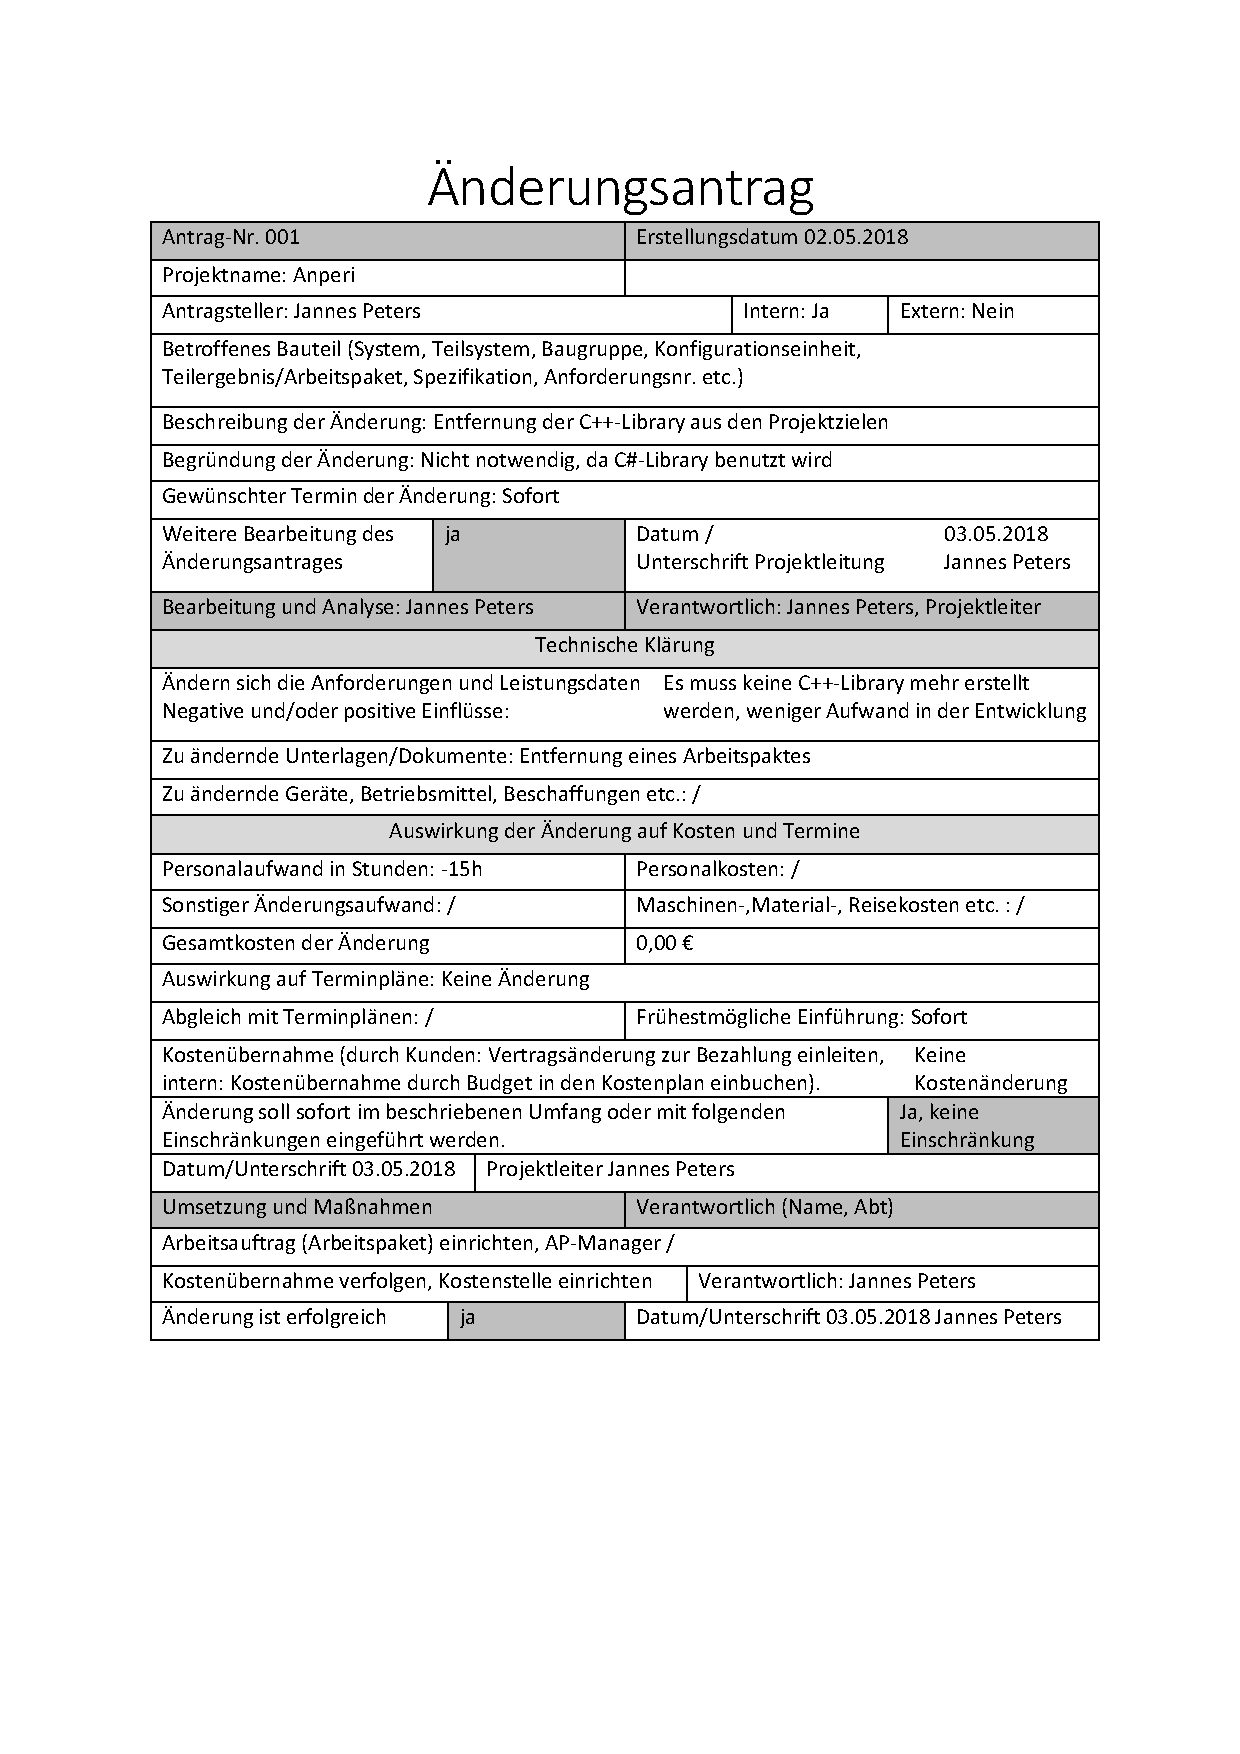
\includegraphics[scale=0.85]{Aenderungsantrag.pdf}
\section{Projektablaufplan}
Alle zwei Wochen wurde der Auftraggeber über den Projektstatus informiert.
Durch diesen Rhythmus entstand eine Bearbeitungsfolge die am besten in Kalenderwochen dargestellt werden kann.
In der folgenden Grafik ist zu erkennen, dass es in nur einem Projektabschnitt einen Verzug gab. Der Verzug ist durch die Abhängigkeit der Java-Library von der C\#-Library entstanden.
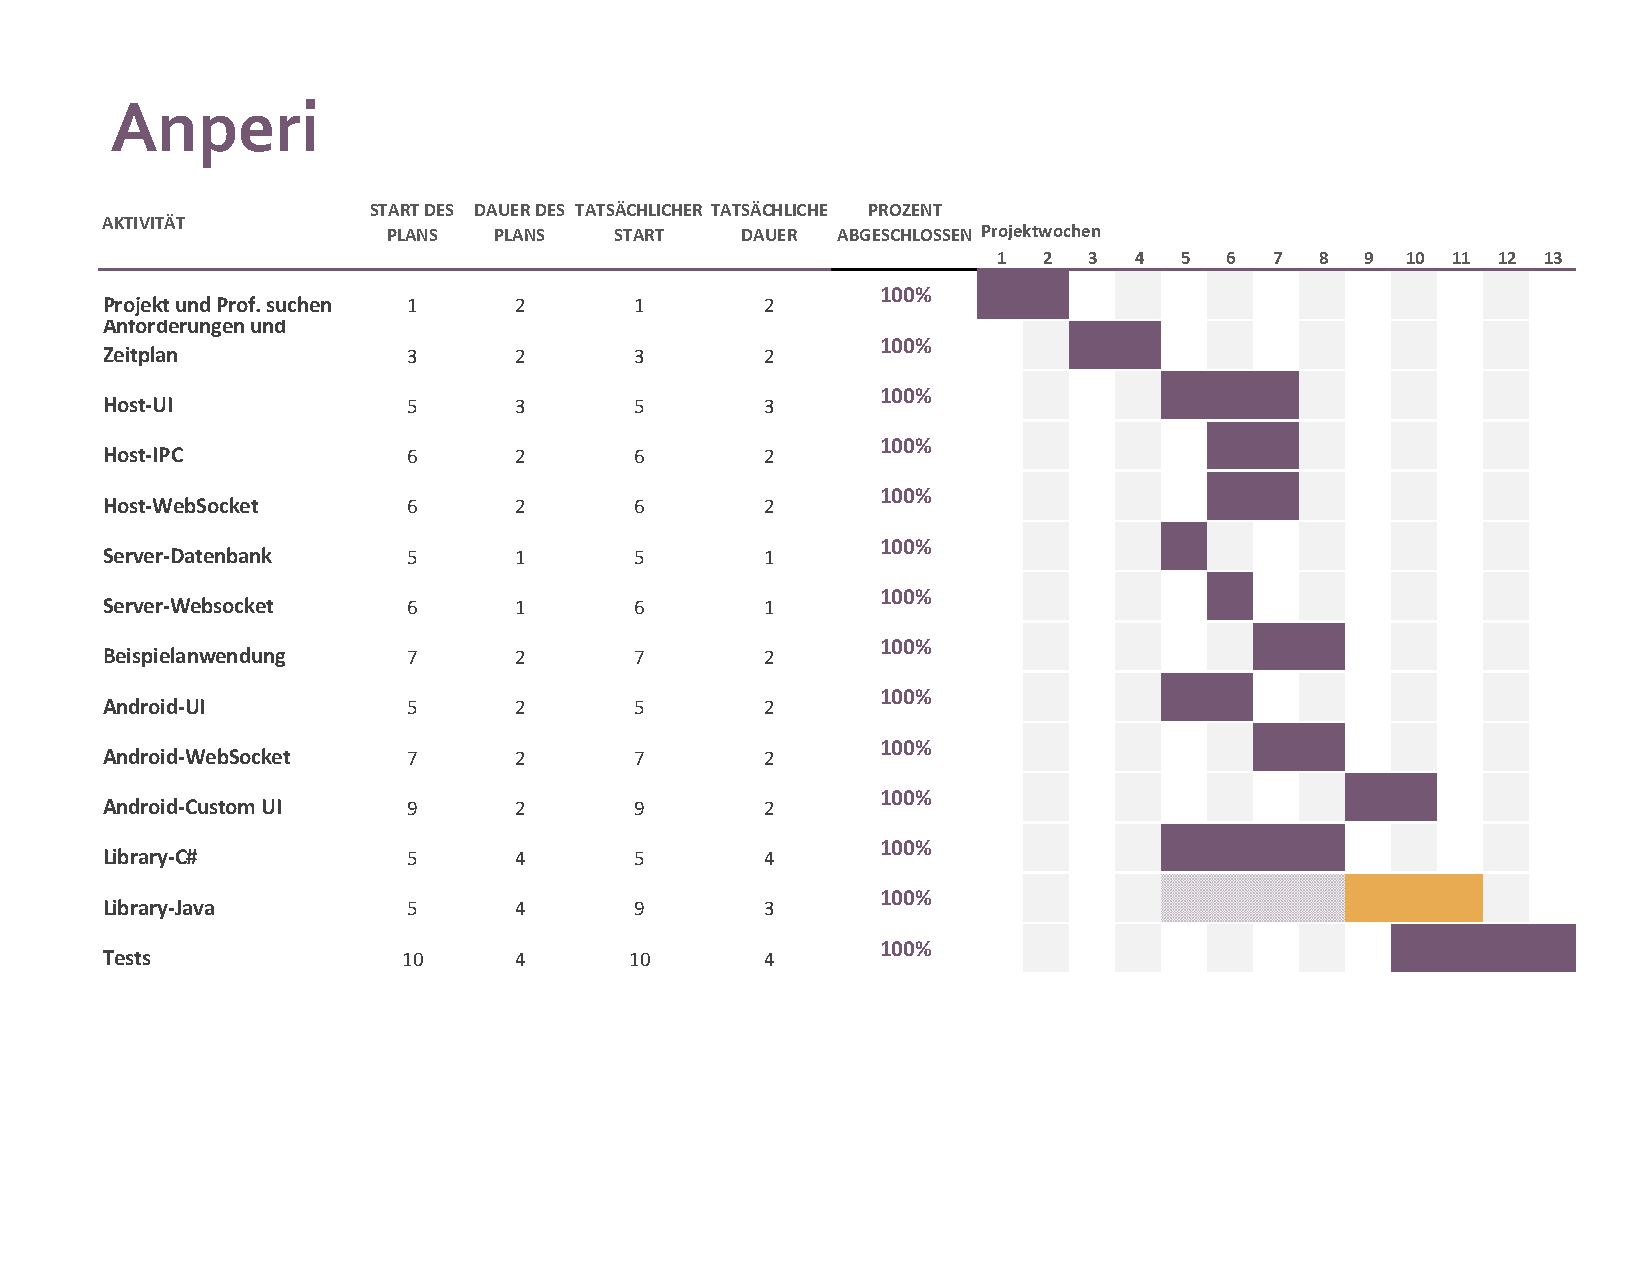
\includegraphics[scale=0.65]{Projektablaufplan.pdf}

\section{Ressourcen- und Kostenplan}
Da das Projekt im Rahmen einer Veranstaltung für das Studium der Projektmitarbeiter stattgefunden hat sind keine Kosten entstanden. \\
Bei dem Projekt handelt es sich um ein reines Softwareprojekt, weshalb keine Ressourcen verbraucht wurden. 

\section{Analyse der Projektergebnisse}

\subsection{Umfang und Qualität}
\subsubsection{Projektbeschreibung}

\textbf{Androidgeräte als PC-Peripherie (I/O-Controller)}\\
Die meisten PC-Nutzer nutzen auch mobile Endgeräte wie Smart­phones oder Tablets. Es existieren bereits Apps, die es ermöglichen, ein Tablet als weiteren (Touch-)Bildschirm an einem PC zu nutzen. Diese Apps sind jedoch in der Regel recht allgemein gehalten.\\
In diesem Projekt soll eine Schnittstelle in Form einer Programmbibliothek (Java/C\#/C++) und einer Android-App als Gegenstück entwickelt werden. Dies soll es unterschiedlicher Software erlauben, durch individuelle Erweiterungen ein Tablet oder Smartphone als Anzeige- und Eingabe­medium zu nutzen und dabei gezielt auf die Anforderungen der zu bedienenden Software einzugehen.\\
\subsubsection{Vergleich mit den Anforderungen}
Dieser Beschreibung wird das umgesetzte Projekt in fast allen Anforderungen gerecht. Neben der wie geforderten Funktionalität der App wurden auch eine Java- und C\#-Library erstellt. Einzig die C++-Library wurde im Verlaufe des Projektes als nicht notwendig eingestuft, da unter C++ auch die C\#-Library benutzt werden kann.
Die Abgegebene Software wurde vielen Tests unterzogen, um eine reibungslose Bedienung zu garantieren.

\subsection{Nachkalkulation}
Es wurden weder Geld noch Ressourcen verbraucht, deshalb wird keine Nachkalkulation aufgestellt.

\section{Beurteilung}
Das Projekt wurde erfolgreich beendet. Das Projektziel wurde vollständig erreicht und gut umgesetzt. Die Zusammenarbeit innerhalb der Gruppe war effektiv, motiviert, zielorientiert und kommunikativ. Auch die Zusammenarbeit mit dem Auftraggeber lief ohne Komplikationen ab, es herrschte ein stetiger Austausch. So konnten Änderungen schnell und effektiv in den Arbeitsprozess einfließen. Sowohl das Projektteam, als auch der Auftraggeber konnten zu jeder Zeit Einwände und Vorschläge eingeben, dadurch konnte eine hohe Zufriedenheit mit dem Endprodukt erreicht werden.

\section{Lessons learned}
\begin{itemize}
	\item {Kommunikation ist einer der wichtigsten Bestandteile einer Projektarbeit (Intern und Extern) }
	\item {Es sollten zu jeder Zeit unterschiedliche Kommunikationskanäle ansprechbar, um einen flüssigen und stetigen Informationsfluss zu ermöglichen}
	\item {Zeitmanagement ist für eine Gruppenarbeit unerlässlich und kann bei richtiger Ausführung das Projekt vor großen Fehlern bewahren}
	\item {Es ist wichtig das Motivationsniveau der Gruppe stetig auf einem hohen Level zu halten, um eine Ermüdung zum Ende der Projektphasen zu vermeiden}
	\item {Offenheit gegenüber anderen/neuen Ideen während des Projektablaufs führt zu einem verbesserten Endprodukt}
\end{itemize}
\end{document}